This step will get the first layer cross, this equals to fitting and orientating of the edges in the yellow face. 
The step is generally described in subsection \ref{sub:step1}.
First the method takes the edge \cubie{} in \cubicle{} \vr{P1S0} (see subsection \ref{sub:cubicle}) 
and checks if the edge \cpiece{} is positioned correctly.
If that is the case and the edge \cpiece{} is orientated correctly, the program proceeds to the next edge \cpiece{}.
If the \cubicle{} is positioned correctly, but not orientated correctly the method will perform an algorithm, which changes the edge \cpiece{}'s orientation without ruining other possibly correctly positioned edge \cpiece{}s. 
This algorithm is named \vr{algorithm 1A}. When the edge \cpiece{} is in the correct position and has the correct orientation, the program moves on to another edge \cpiece{}. 

If the edge \cpiece{} is not in its correct position, then the method checks where the \cpiece{} is positioned. 
Depending on which layer it is in, different actions will be taken:
\begin{enumerate}
	\item If the edge \cpiece{} in question is in the first layer it is moved to the opposite layer.
	\item If the edge \cpiece{} is positioned in the second layer an algorithm is performed, which moves the edge \cpiece{} to the last layer, which is the opposite of the layer in which we make the cross. This algorithm is called \vr{algorithm 1B} (see code snippet \ref{src:middleMove}). 
	The algorithm takes a \cubicle{} as input and performs a specific move sequence accordingly.
	The move sequences in the different cases are generally the same, but since we only view the \rubik{} from one angle, we have to move different faces in the move sequence accordingly to the cubicle which is input. e.g. if the cubicle is in the front and right faces the move sequence is performed as it originally is. 
	However when the cubicle is in the right and back faces, every move will rotate 90 degrees, so that an \m{F} move becomes a \m{R} move etc.
	\item If the edge \cubie{} is in the last layer, no action is performed, since this is where we want it to be for now.
\end{enumerate}

In the \textbf{for} loop, in code snippet \ref{src:middleMove}, the moves are added to an array, which purpose is to write the moves in the GUI console. 
The \vr{Cube.permute} method applies the moves to the cube.

\begin{lstlisting}[style=sourceCode, caption=\myCaption{This is algorithm 1B, which will move an edge piece from the middle layer to the top layer without ruining any edge pieces which are correctly positioned in the cross.}, label=src:middleMove, float=htb]
private void algorithm1B(EdgePos p){
	MoveButtons[] moves;
	switch (p) {
	case S0T0:
		moves = new MoveButtons[]{ F, U, FP};
		break;
	case S0T1:
		moves = new MoveButtons[]{ FP, U, F};
		break;
	case S1T0:
		moves = new MoveButtons[]{ BP, U, B};
		break;
	default:
		moves = new MoveButtons[]{ B, U, BP};
		break;
	}
	for(int i = 0; i < moves.length; i++){
		this.moves.add(moves[i]);
	}
	Cube.permute(cube, moves);
}
\end{lstlisting}

Now that the edge \cpiece{} is in the last layer it needs to be moved to the position directly above where it is correctly positioned. 
The program does this by applying an \m{U} \twist{} and checking if the edge \cpiece{} is above its correct position.
The edge \cpiece{} is now positioned in the last layer face and the face which has the same color as the edge  \cpiece{}'s other \facelet{} i.e. the \facelet{} that is not yellow.
In order to position the edge \cpiece{} correctly that face is twisted twice.
The edge \cpiece{} is now in it's correct position, and if it is orientated correctly the program moves on to another edge \cpiece{} .
If the edge \cpiece{} is oriented incorrectly \vr{algorithm 1A} is performed. If more edge \cpiece{}s need to be positioned or oriented correctly the program will continue with the same method until the cross is finished in which case the program moves on to the next step. See figure \ref{fig:FlCrossFlow}.

\begin{figure}[htbp]
	\centering
		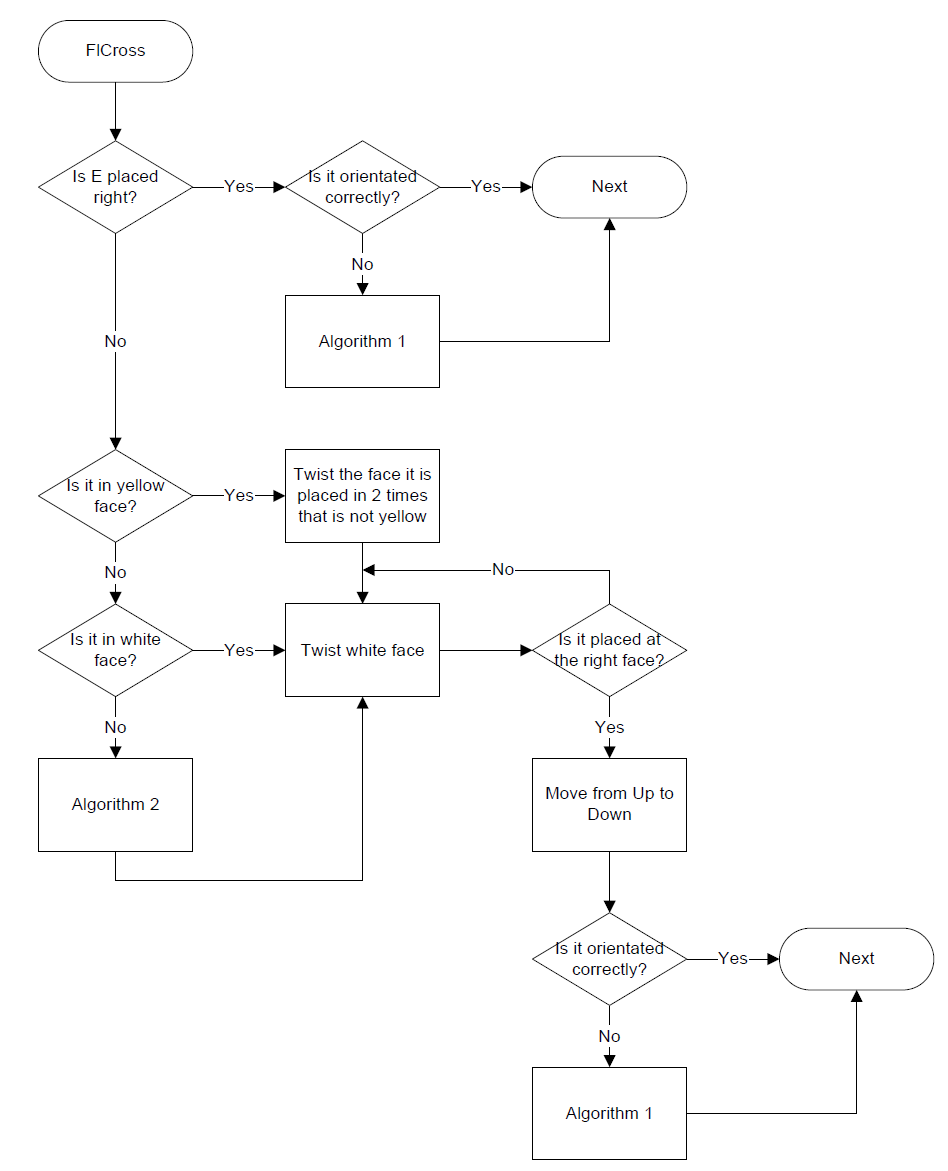
\includegraphics[width = \textwidth]{input/pics/FlCrossFlow3.png}
	\caption{\myCaption{The figure illustrates what is done in step 1.}}
	\label{fig:FlCrossFlow}
\end{figure}

